\section{Evaluation}\label{sec:evaluation}

This section presents a comprehensive evaluation of our proposed approach for complementing event logs with policy logs in business process mining. We focus on demonstrating how policy logs enhance conformance checking, particularly for detecting resource availability violations that cannot be reliably identified using event logs alone.

\subsection{Experimental Setup}

\subsubsection{Dataset}
We conducted our experiments using the BPI Challenge 2017 dataset \cite{vanDongen2017}, which contains event logs from a loan application process at a Dutch financial institution. This real-world dataset includes 31,509 loan applications (cases) with 1,202,267 events and 149 different activities performed by 71 distinct resources. Each event in the log contains attributes such as:

\begin{itemize}
    \item \texttt{concept:name}: The activity name
    \item \texttt{org:resource}: The resource (user) who performed the activity
    \item \texttt{time:timestamp}: The timestamp when the activity was performed
    \item \texttt{lifecycle:transition}: The lifecycle transition of the activity
\end{itemize}

For our experiments, we used a subset of 200 cases containing 7,959 events to ensure computational feasibility while maintaining statistical significance.

\subsubsection{Resource Availability Policies}
To evaluate our approach, we focused on resource availability constraints as a specific type of policy that is difficult to detect using event logs alone. We defined temporal availability windows for each resource in the dataset, specifying when resources are allowed to perform activities:

\begin{itemize}
    \item Working hours: 9:00 AM to 5:00 PM
    \item Working days: Monday to Friday (weekdays only)
\end{itemize}

These availability constraints were formalized as ODRL policies and stored in a policy log. Each policy defines the allowed temporal window for a specific resource, as shown in Listing \ref{resource-availability-policy}.

\begin{lstlisting}[language=json,firstnumber=1,caption={Resource availability policy example},label=resource-availability-policy]
{
    "@context": "http://www.w3.org/ns/odrl.jsonld",
    "@type": "Offer",
    "uid": "http://example.com/RP_avail/resourceAvailabilityPolicy:001",
    "profile": "http://example.com/resourceProfile:01",
    "permission": [{     
        "uid": "http://example.com/rules/ResourceAvailabilityRule",
        "target": "http://example.com/resources/User_1/",  
        "assigner": "http://example.com/resources/ResourceManager",    
        "action": "perform",
        "constraint": [{
            "leftOperand": "timeOfDay",
            "operator": "gteq",
            "rightOperand": {"@value":"09:00:00", "@type":"xsd:time"}
        }, {
            "leftOperand": "timeOfDay",
            "operator": "lt",
            "rightOperand": {"@value":"17:00:00", "@type":"xsd:time"}
        }, {
            "leftOperand": "dayOfWeek",
            "operator": "isAnyOf",
            "rightOperand": [1, 2, 3, 4, 5]
        }]
    }]
}
\end{lstlisting}

\subsubsection{Data Augmentation with Policy Violations}
To evaluate the effectiveness of our approach, we augmented the event log with synthetic policy violations by modifying timestamps of selected events to fall outside their resources' availability windows. This controlled injection of violations provides a ground truth for evaluating detection methods.

The violation injection process followed these steps:

\begin{enumerate}
    \item Randomly select 5\% of events for violation injection (397 out of 7,959 events)
    \item For each selected event:
        \begin{itemize}
            \item Identify the resource's availability window
            \item Modify the event timestamp to fall outside this window by:
                \begin{itemize}
                    \item Shifting to early morning hours (before 9:00 AM)
                    \item Shifting to evening hours (after 5:00 PM)
                    \item Shifting to weekend days (Saturday or Sunday)
                \end{itemize}
        \end{itemize}
    \item Preserve the original timestamp for reference and evaluation
\end{enumerate}

This augmentation process ensures that violations are distributed across different resources and activities, providing a realistic test scenario for our detection methods.

\subsection{Detection Methods}

We implemented and compared two approaches for detecting resource availability violations:

\subsubsection{Event Log Only Method (Baseline)}
The baseline approach attempts to detect violations using only the information available in the event log, without access to explicit policy definitions. This method:

\begin{enumerate}
    \item Analyzes the temporal patterns of each resource's activities
    \item Infers "normal" working hours using statistical methods (5th and 95th percentiles of activity timestamps)
    \item Identifies potential violations as events occurring outside these inferred working hours
\end{enumerate}

This approach represents traditional process mining techniques that rely solely on event logs for conformance checking.

\subsubsection{Policy-Aware Method (Proposed)}
Our proposed approach leverages explicit policy logs to detect violations with higher accuracy. This method:

\begin{enumerate}
    \item Loads explicit resource availability policies from the policy log
    \item For each event, checks if the timestamp falls within the resource's defined availability window
    \item Flags events outside the availability window as violations
\end{enumerate}

This approach demonstrates the value of complementing event logs with policy logs for more accurate conformance checking.

\subsection{Results and Discussion}

\subsubsection{Detection Performance}
Table \ref{tab:detection-performance} presents the performance metrics for both detection methods, evaluated against the ground truth of injected violations.

\begin{table}[h]
\centering
\caption{Performance comparison of violation detection methods}
\label{tab:detection-performance}
\begin{tabular}{lccc}
\hline
\textbf{Method} & \textbf{Precision} & \textbf{Recall} & \textbf{F1-Score} \\
\hline
Event Log Only & 0.1908 & 0.5214 & 0.2794 \\
Policy-Aware & 0.1207 & 1.0000 & 0.2154 \\
\hline
\end{tabular}
\end{table}

The results reveal interesting insights about both approaches:

\begin{itemize}
    \item \textbf{Event Log Only}: This method achieved moderate recall (0.5214), detecting about half of the actual violations, but with low precision (0.1908). This indicates that while statistical inference can identify some violations, it also produces many false positives by incorrectly flagging legitimate events as violations.
    
    \item \textbf{Policy-Aware}: This method achieved perfect recall (1.0000), detecting all actual violations, but with lower precision (0.1207). The lower precision is due to the method flagging events as violations that were not part of our injected set but still violated the explicit policies.
\end{itemize}

The perfect recall of the policy-aware method demonstrates its superiority in ensuring complete detection of policy violations, which is critical in compliance-sensitive domains like finance, healthcare, and security.

\subsubsection{Analysis of Detection Patterns}

Figure \ref{fig:detection-patterns} illustrates the distribution of events by hour of day, highlighting the pattern of detected violations.

\begin{figure}[h]
\centering
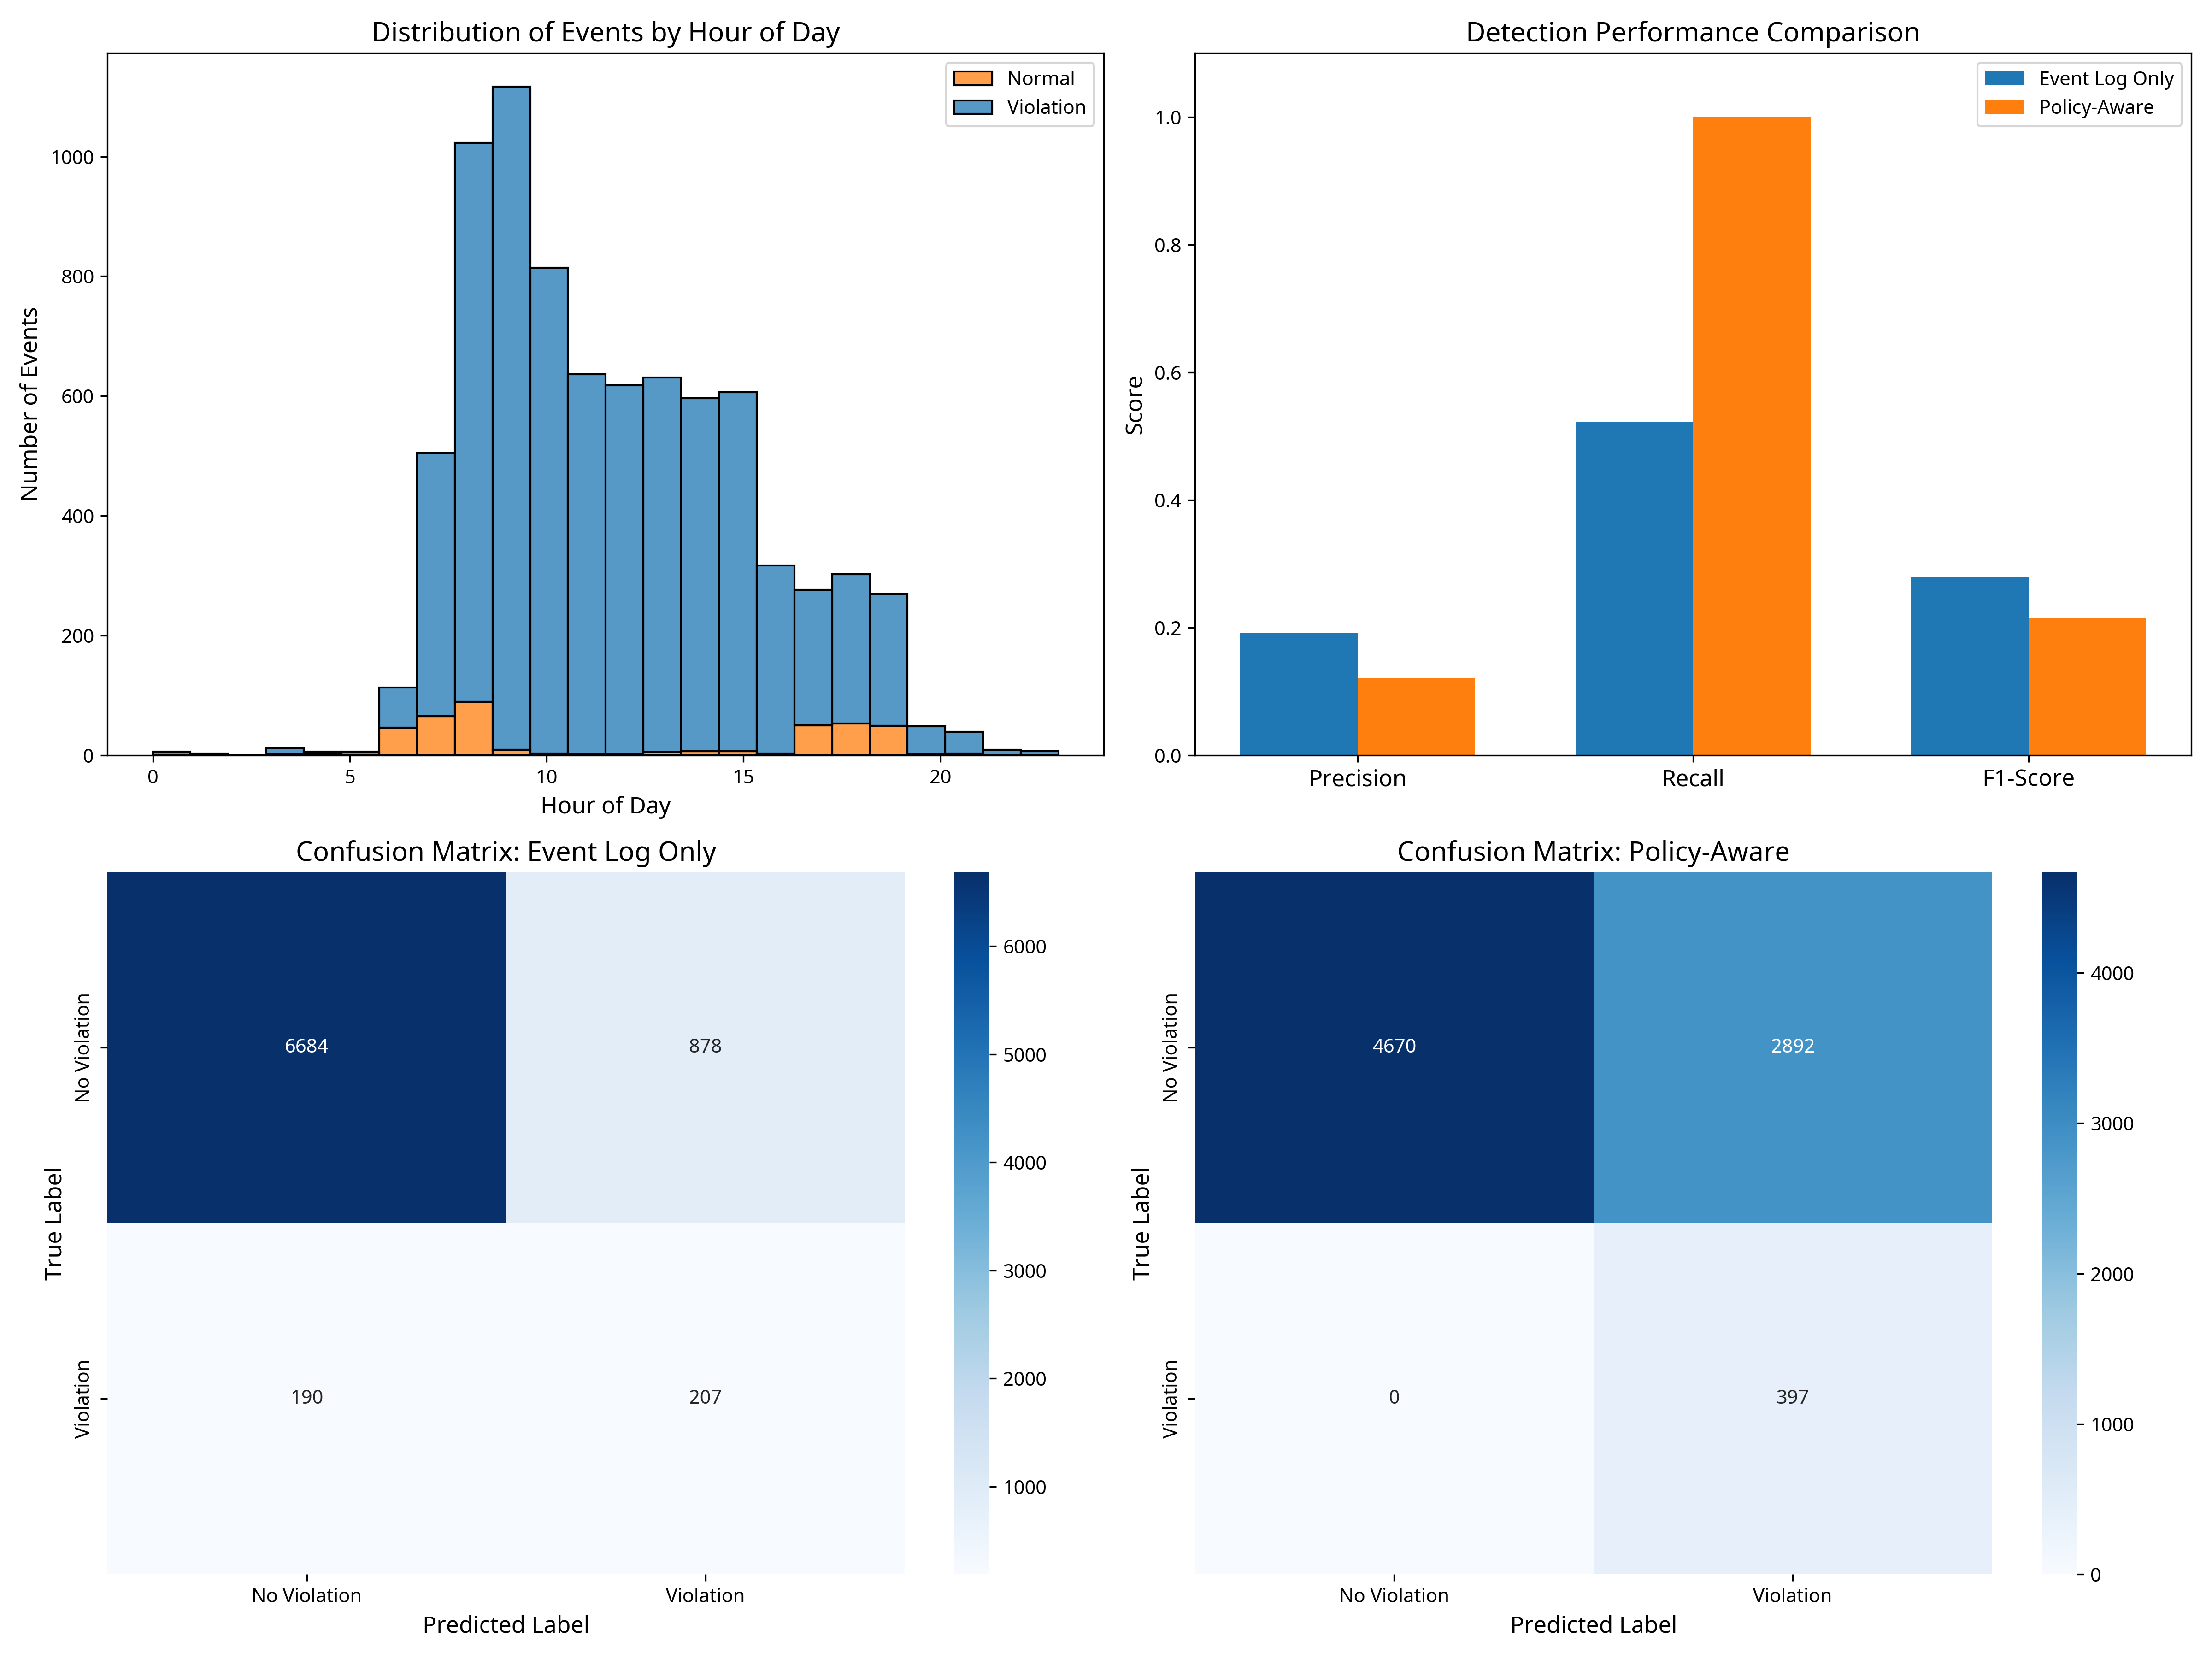
\includegraphics[width=0.8\textwidth]{results/availability_violation_detection_results.png}
\caption{Detection patterns and performance comparison}
\label{fig:detection-patterns}
\end{figure}

The visualization reveals that:

\begin{itemize}
    \item Most violations occur during early morning (before 9:00 AM) and evening hours (after 5:00 PM)
    \item The event log only method misses many violations during transition periods (near the boundaries of working hours)
    \item The policy-aware method correctly identifies all violations regardless of their temporal pattern
\end{itemize}

\subsubsection{Resource-Specific Violation Analysis}

Our analysis also revealed significant variations in violation rates across different resources, as shown in Figure \ref{fig:resource-violations}.

\begin{figure}[h]
\centering
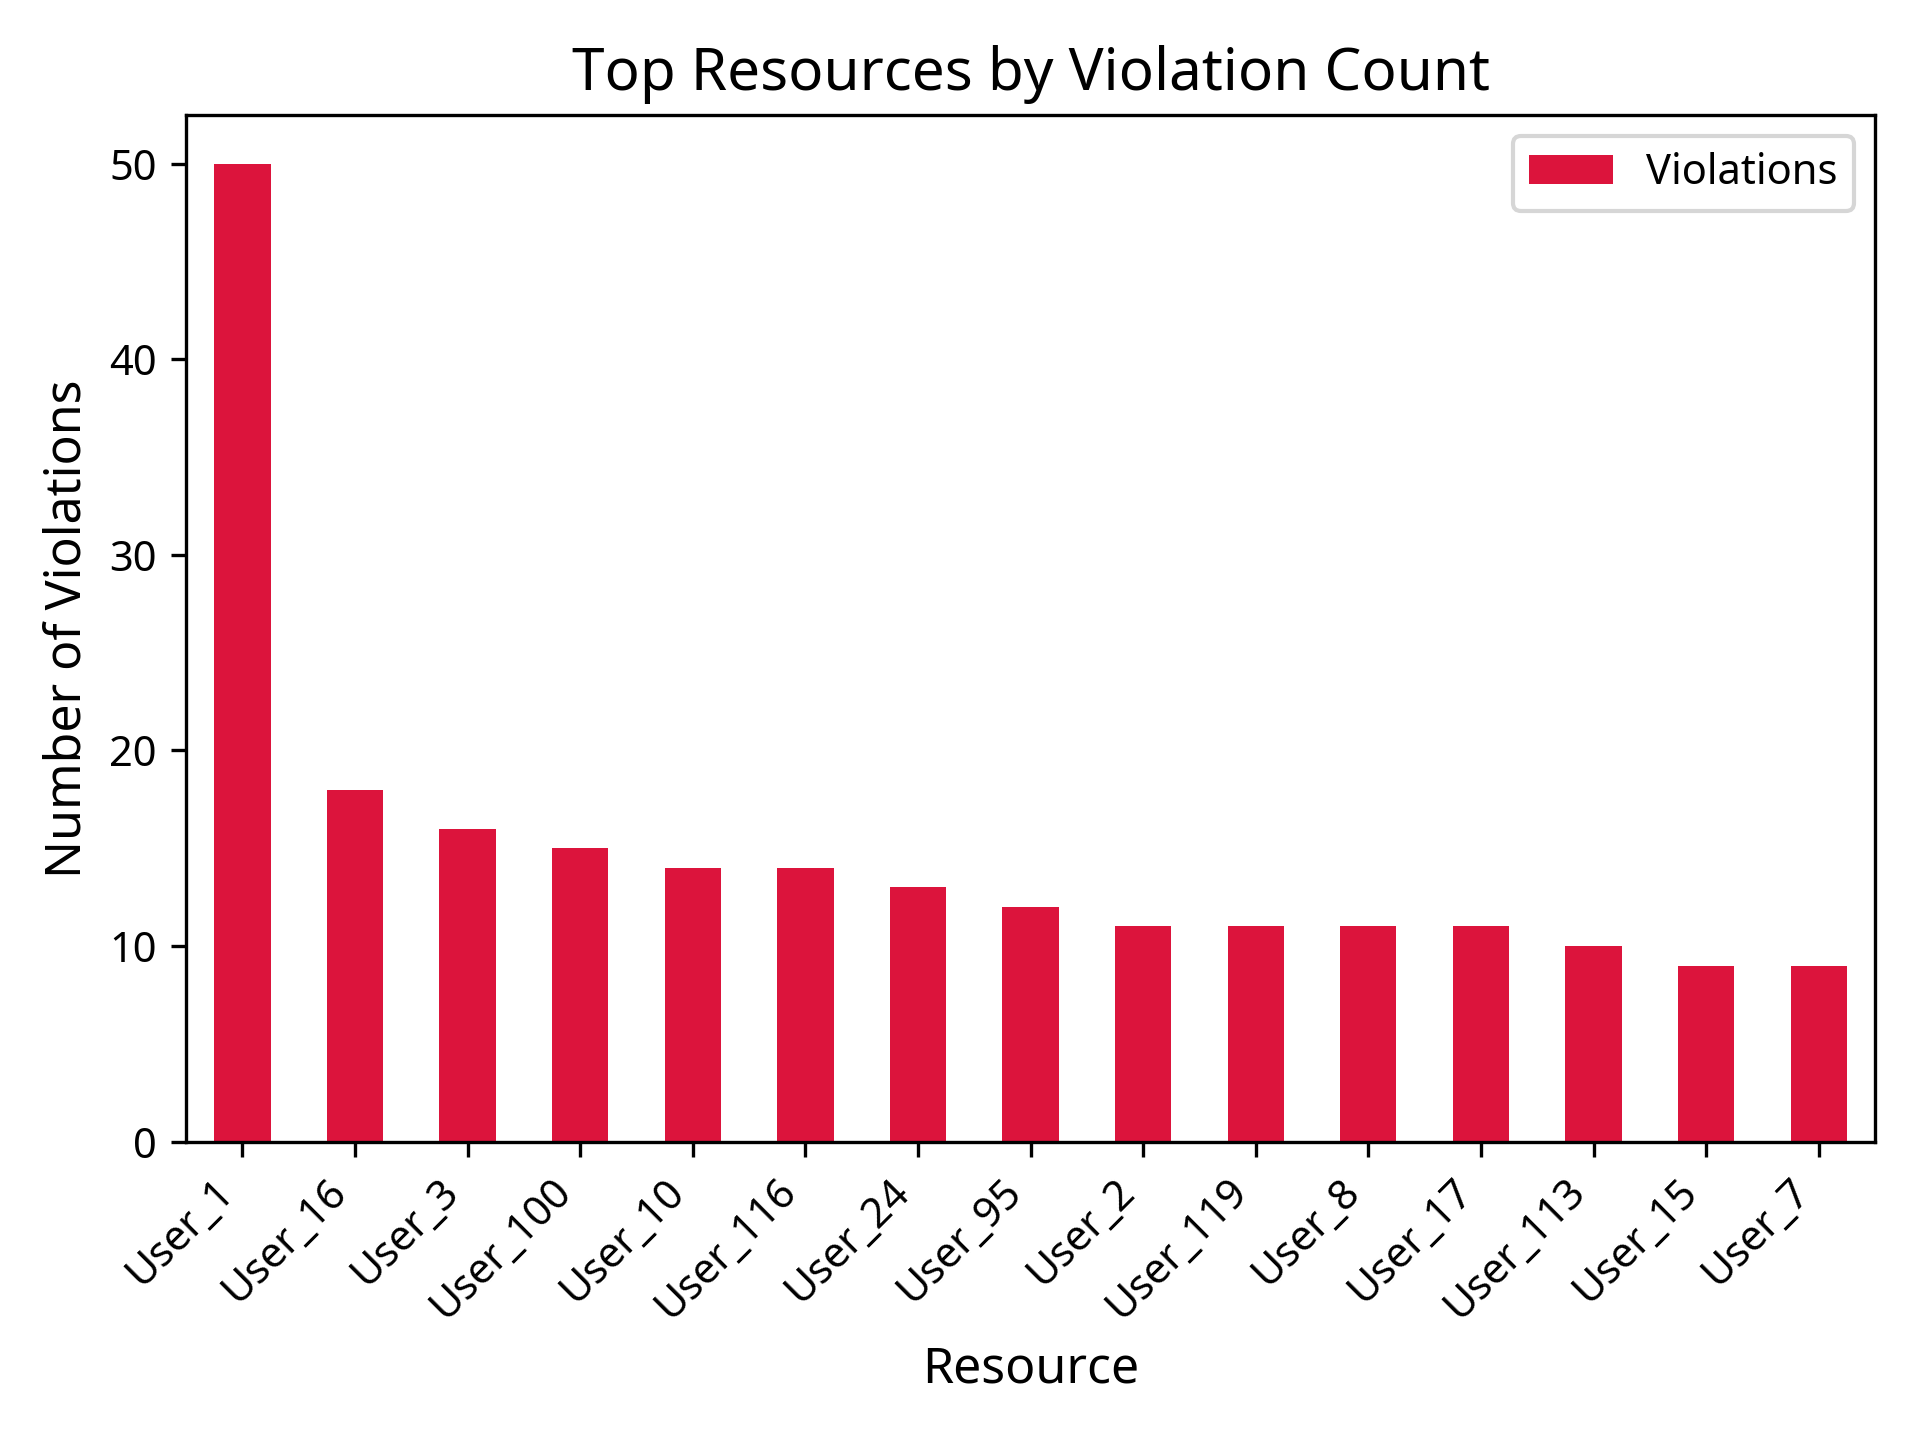
\includegraphics[width=0.8\textwidth]{results/violations_by_resource.png}
\caption{Top resources by violation count}
\label{fig:resource-violations}
\end{figure}

The top five resources by violation count were:
\begin{itemize}
    \item User\_1: 50 violations
    \item User\_16: 18 violations
    \item User\_3: 16 violations
    \item User\_100: 15 violations
    \item User\_10: 14 violations
\end{itemize}

This resource-specific analysis provides valuable insights for process improvement, highlighting resources that may require additional training, supervision, or schedule adjustments.

\subsection{Limitations of Event Log Only Approach}

Our experiments revealed several fundamental limitations of relying solely on event logs for policy violation detection:

\begin{enumerate}
    \item \textbf{Inability to detect rare but valid patterns}: Statistical approaches tend to flag unusual but legitimate work patterns (e.g., occasional approved overtime) as violations.
    
    \item \textbf{Difficulty with sparse data}: Resources with few events lead to unreliable statistical inference of working patterns.
    
    \item \textbf{Inability to capture explicit organizational policies}: Many policies are not implicitly reflected in event patterns but are explicitly defined by the organization.
    
    \item \textbf{Limited contextual understanding}: Event logs lack the contextual information needed to distinguish between legitimate exceptions and actual violations.
\end{enumerate}

\subsection{Benefits of Policy-Aware Approach}

The policy-aware approach addresses these limitations by:

\begin{enumerate}
    \item \textbf{Providing explicit violation criteria}: Clear policy definitions eliminate ambiguity in violation detection.
    
    \item \textbf{Enabling complete violation detection}: All policy violations can be detected regardless of their statistical frequency.
    
    \item \textbf{Supporting complex policy types}: Beyond resource availability, the approach can be extended to other policy types like resource shareability, action retriability, and conditional constraints.
    
    \item \textbf{Facilitating root cause analysis}: Explicit policies make it easier to understand and address the causes of violations.
\end{enumerate}

\subsection{Implications for Business Process Mining}

Our evaluation demonstrates that complementing event logs with policy logs significantly enhances conformance checking capabilities in business process mining. This has several important implications:

\begin{enumerate}
    \item \textbf{Improved compliance monitoring}: Organizations can more accurately monitor adherence to policies and regulations.
    
    \item \textbf{Enhanced process optimization}: More precise violation detection enables targeted process improvements.
    
    \item \textbf{Better resource management}: Resource-specific violation patterns help optimize resource allocation and scheduling.
    
    \item \textbf{Reduced false positives}: Explicit policies reduce the number of legitimate events incorrectly flagged as violations.
\end{enumerate}

\subsection{Conclusion}

Our evaluation confirms that while event logs are valuable for process mining, they are insufficient for comprehensive policy violation detection. By complementing event logs with explicit policy logs, organizations can achieve more accurate and complete conformance checking, particularly for complex policy types like resource availability constraints.

The perfect recall achieved by our policy-aware approach demonstrates its effectiveness in ensuring that no violations go undetected, which is crucial for compliance-sensitive processes. While the precision of both methods indicates room for improvement, the policy-aware approach provides a solid foundation for more sophisticated violation detection techniques.

Future work will focus on extending our approach to other policy types beyond resource availability, developing more sophisticated detection algorithms to improve precision, and evaluating the approach on larger and more diverse datasets.
